% background
% brief review of previous research (cite)
% reson why the research was undertaken
% Hypothesis
% explenation of techniques and why they ve been chosen
% objectives = what you hope to achieve
% brief reference to the main outcome

%$\ce{CdS_x Se_{1-x}/ZnS}$

% \begin{figure*}
%   \centering
%   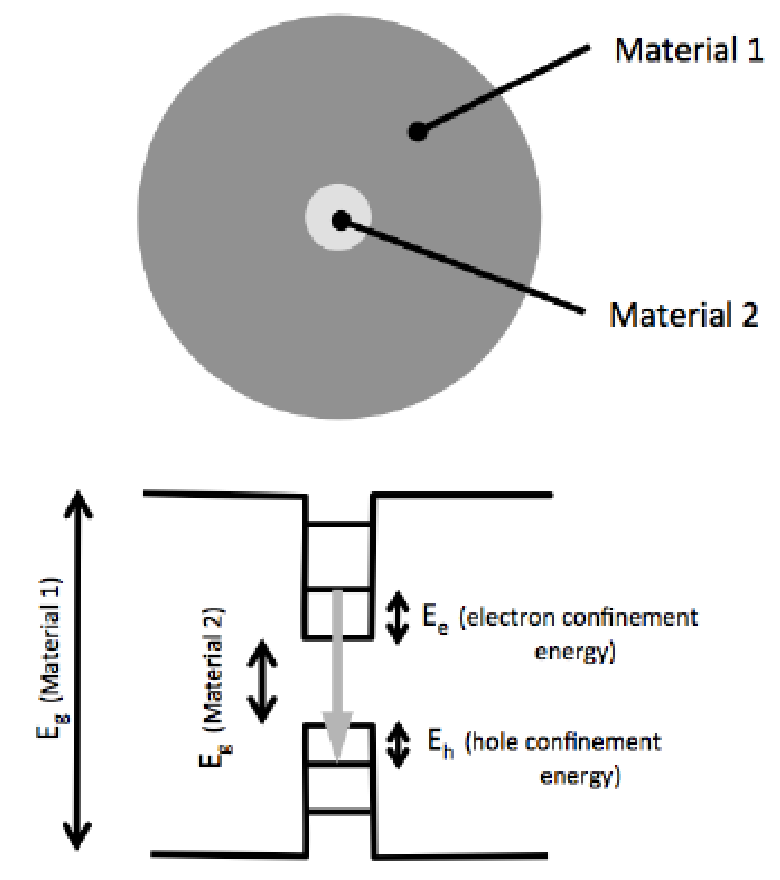
\includegraphics[width=0.35\textwidth]{graphics/QD.png}
%   \caption[width=0.4\textwidth]{\cite{instruction}.}
%   \label{fig:QD}
% \end{figure*}

\section{Introduction}
\label{sec:Introduction}

X-ray fluorescence is the emission of secondary, element characteristic x-rays due to an exctation by high-energy X- or gammarays.
So, by comparing the fluorescence spectrum of an unknown sample with the spectra of known ones, the specimen can be easily identified.
Further, by X-ray diffraction the christallography can be analyzed, as the diffraction pattern depends on the lattice parameters.
In more detail, the scattering potential, and thus the electons density of the threedimensional sample has a characteristic diffraction pattern.
From this, the atoms positions, the chemical bonds and also christallographic disorders can be determined.

\subsection{Experimental setup}
\label{sec:setup}

For the fluorescence measurement a high-energy X-ray source $\ce{^{133}Ba}$ is used. 
The sample (Sample B) is positioned in a sample holder between the source and a $\ce{Si}$ detector as depicted schematically in figure \ref{fig:setup}.
This is connected with a multichannelanalyzer and then with a PC.
It is important to notice that the X-ray source is $\ce{^{133}Ba}$ and thus decays into $\ce{Cs}$ by electron capture.
Thus, the main emitted X-ray signal is at the energy of the $\alpha$ peak of $\ce{Cs}$, which is $\SI{30.972}{\kilo\eV}$ \cite{Ba-source}.

In detail the used instruments are
\begin{itemize}
    \item $\ce{^{133}Ba}$ X-ray source
    \item AMPTEK XR-100CR Si-based X-ray detector
    \item Multichannelanalyzer
    \item Data analysis software PANalytical X`Pert HighScore
\end{itemize}
The diffraction measurement is done on a rotatable stage, where also a monochromator is introduced between the sample and the detector.

\begin{figure*}
    \centering
    \captionsetup{width=0.9\linewidth}
    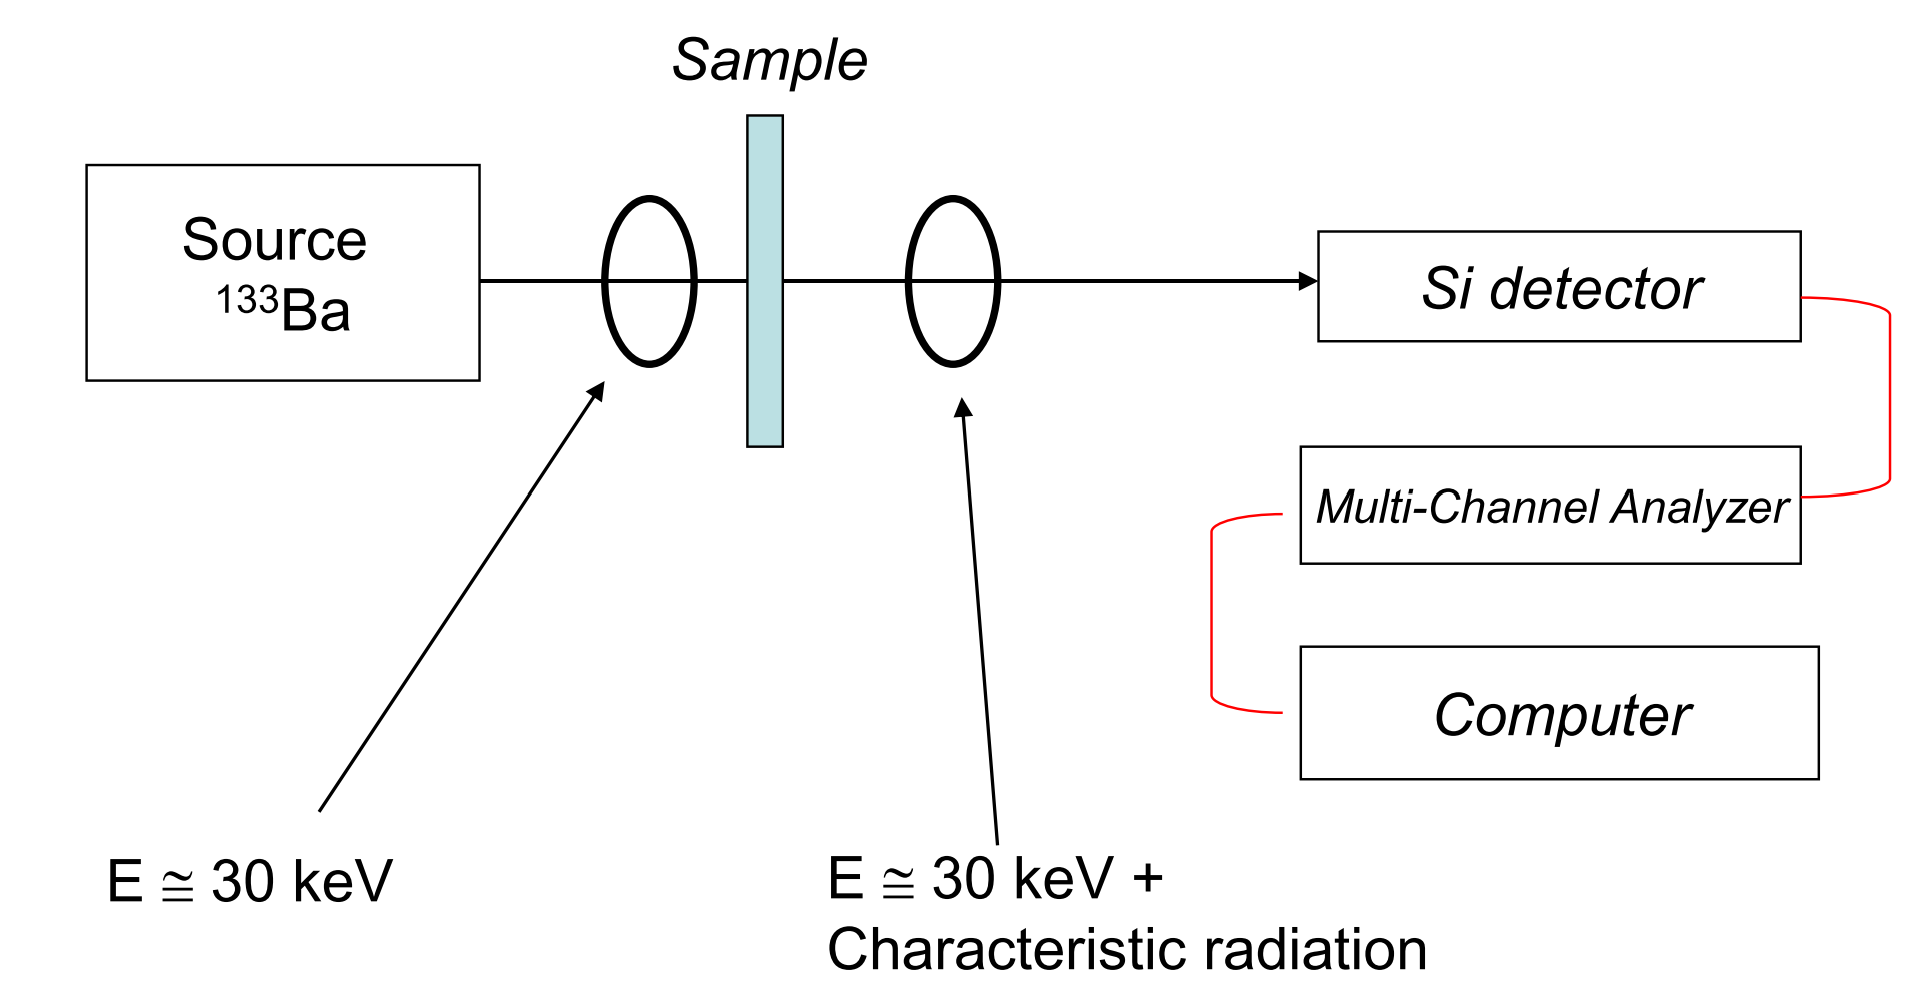
\includegraphics[width=0.8\textwidth]{graphics/setup.png}
  \caption{Schematic setup of a X-ray fluorescence erperiment, where the sample is positioned between the source and a X-ray Si detector. This is connected to a analysis PC software through a MCA \cite{instruction}.)}
    \label{fig:setup}
\end{figure*}

\subsection{Energy scaling}
\label{sec:E_scaling}
As the output of the multichannelanalyzer (MCA) is counts per bin, but one wants to refer the wavelegth and thus an energy out of the channel, 
spectral measurements for several samples are done.
The characteristic spectral peak of the sample is found, so that tuples of bin number and energy can be found.
By a linear regression a function $E (\text{b})$  of the bin $b$ can be found.
